%!TEX program = lualatex
\documentclass[xcolor={dvipsnames}]{beamer}
\usepackage[T1]{fontenc}
\usepackage[english]{babel}
\usepackage{amssymb}
\usepackage{amsmath}
\usepackage{tikz}
\usepackage{xcolor}
\usepackage{colortbl}
\usepackage{listings}
\usepackage{graphicx}
\renewcommand*\footnoterule{}
\graphicspath{ {./figures/} }


\date{February 23, 2023}
\author{Til Roth}
\title{Can I Opt Out Yet? \\GDPR and the Global Illusion of Cookie Control}
\setbeamertemplate{footline}[page number]
\usetheme{metropolis}
\institute{Hot Topics in Data Networks WS22/23\\Saarland Informatics Campus}

\begin{document}
\maketitle

\section{Motivation}

\begin{frame}
    \centering
    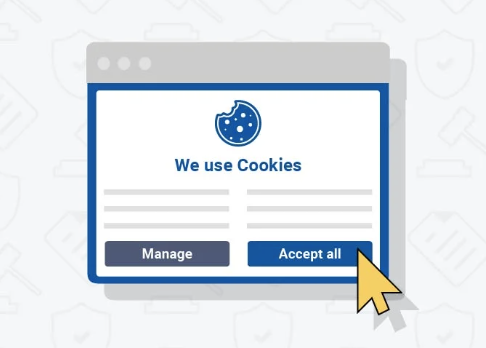
\includegraphics[scale=0.6]{example_notice.png}
\end{frame}

\begin{frame}{Cookie Consent Notices}
	\begin{itemize}
		\item present on many websites
		\item enabling privacy control
		\item result of the \emph{General Data Protection Regulation} (GDPR) issued by the European Union in 2018
	\end{itemize}
\end{frame}

\begin{frame}{GDPR}
	\begin{itemize}
		\item regulate data usage online for EU citizens
        \item specify how user data should be handled
        \item users should be able to \emph{opt-out} of tracking
		\item privacy policies should be readable
	\end{itemize}

    \pause
    \textbf{General research goal}:

    \begin{center}
        evaluate the impact of the GDPR in the EU
    \end{center}

    \pause
    \textbf{Our goal}:

    \begin{center}
        evaluate the impact of the GDPR on an international scale
    \end{center}


    \pause
    Foresight: \approx 90\% of website perform tracking without consent
\end{frame}

\begin{frame}{Outline}
    \begin{itemize}
        \item Technical Background
        \item Methodology
        \item Analysis
    \end{itemize}
\end{frame}

\section{Technical Background}

\begin{frame}{Cookies}
    \begin{itemize}
        \item mechanism for stateful HTTP
        \hspace{5em}
        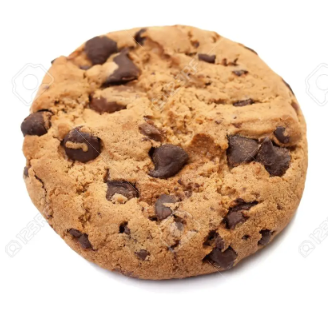
\includegraphics[scale=0.1]{cookie_trans.png}
        \item small item with
            \begin{itemize}
                \item name
                \item value
                \item corresponding URL
                \item time to live
            \end{itemize}
        \item stored in users browser and sent along requests
        \item server can identify user in subsequent visits
        \item enable convenient features like shopping carts
    \end{itemize}
    \footnotesize
    \centering
    \begin{tabular}{ l r }
        name & sessionid \\\hline
        value & 123abc456def789 \\\hline
        URL & example.org \\\hline
        valid & Tue, 16 May 2023 18:08:34 GMT
    \end{tabular}
\end{frame}

\begin{frame}{Cookie Tracking}
    $\rightarrow$ third-party sets unique cookie on user A on visit of foo.com

    $\rightarrow$ third-party sees same cookie on bar.com again

    $\rightarrow$ knows it's user A

    $\rightarrow$ reconstruct browsing history and surfing behavior

    $\rightarrow$ show personalized ads
\end{frame}

\begin{frame}{GDPR}
    \begin{itemize}
        \item applies to data that can uniquely identify a user\\(except essential cookies e.g. shopping cart)
        \item consent must be explicit
        \item data stored not longer than necessary
        \item privacy policies transparent and accessible
        \item applies to any data handling of EU citizens\\(not only EU websites)
    \end{itemize}
\end{frame}

\section{Methodology}

\begin{frame}{Setup}
	\begin{itemize}
		\item AWS Alexa top-1M websites
		\item 2000 websites of the top categories determined by Symantec RuleSpace
	\end{itemize}
\end{frame}

\begin{frame}{Data Collection}
    \begin{itemize}
        \item manual analysis
        \item browser extension to collect the cookies
        \item always opt-out if possible
        \item different types of cookie notices:
            \begin{itemize}
                \item \emph{Anyway}
                \item \emph{AutoAccept}
                \item \emph{OnlyAccept}
                \item \emph{AcceptReject}
                \item \emph{JustSettings}
            \end{itemize}
    \end{itemize}
\end{frame}

\begin{frame}{Identifying Tracking Cookies}
    Common approach:
    \begin{itemize}
        \item known third-party tracker list
        \item probe cookie against list
    \end{itemize}

    \pause
    \vspace{2em}

    Approach of the underlying work:
    \begin{itemize}
        \item with xzcvbn (password strength tool)
        \item entropy of the cookie value
            \begin{itemize}
                \item "german" $\rightarrow$ no tracker
                \item "1283762761628371628317263817263" $\rightarrow$ tracker
            \end{itemize}
        \item afterwards use third-party tracker list to distinguish between third-party and first-party trackers
    \end{itemize}
\end{frame}

\begin{frame}{Privacy Policies}
    \begin{itemize}
        \item copy HTML of the privacy policy of website upon visit
        \item evaluate reading difficulty with two metrics
            \begin{itemize}
                \item Flesch Reading Ease Score (FRES)
                \item Flesch-Kincaid Reading Level (FKRL)
        \end{itemize}
    \end{itemize}
\end{frame}

\section{Analysis}

\begin{frame}{Type of Tracking}
    \centering
    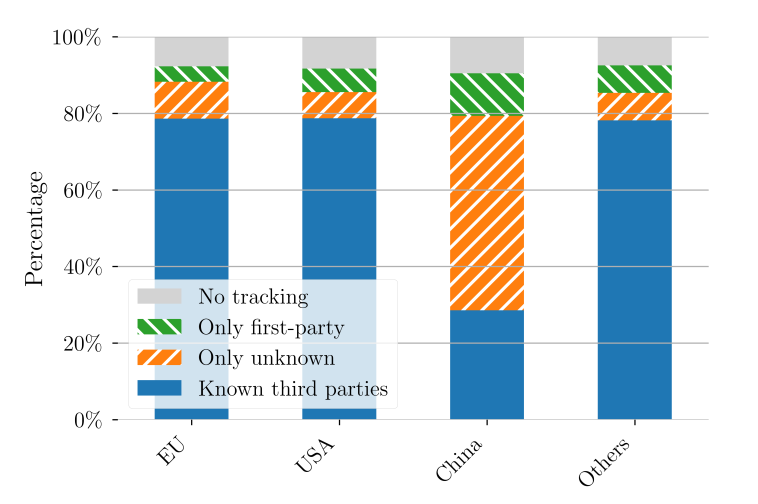
\includegraphics[scale=0.36]{figures/tracking_kind_trans.png}
\end{frame}

\begin{frame}{Size of Consent Notice}
    \centering
    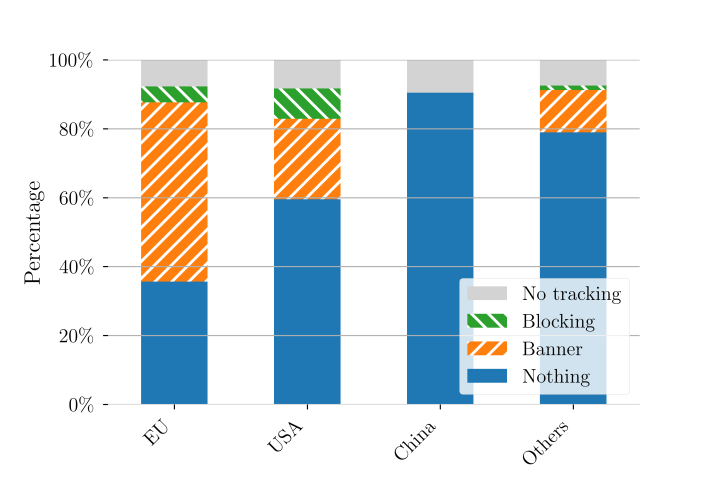
\includegraphics[scale=0.4]{figures/cookie_notice_size_trans.png}
\end{frame}

\begin{frame}{Type of Consent Notice}
    \centering
    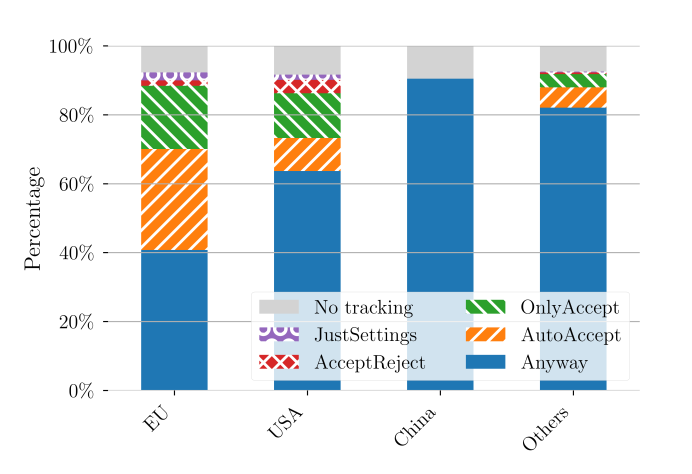
\includegraphics[scale=0.4]{figures/cookie_notice_type_trans.png}
\end{frame}

\begin{frame}{Third-Party opt-out}
    \centering
    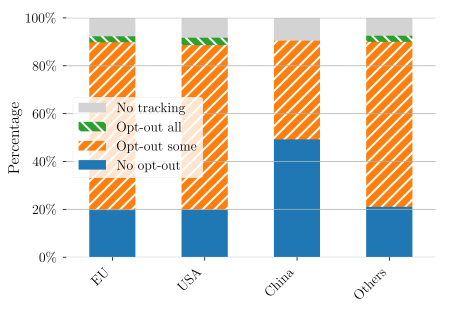
\includegraphics[scale=0.58]{figures/third_party_trans.png}
\end{frame}

\begin{frame}{Privacy Policies}
    Underlying work of 2019:\\
    \vspace{.5em}
    \centering
    \begin{tabular}{ l r r r }
        \hline
        Region & Policies & FRES & FKRL \\
        \hline
        EU & 190 & 57.1 & 10.5 \\
        USA & 617 & 54.5 & 11.2 \\
        All & 849 & 54.1 & 11.1 \\
        \hline
    \end{tabular}

    \vspace{1em}

    \begin{tabular}{ l r r }
        \hline
        & FRES & FKRL \\
        \hline
        2004 & 34.2 & 14.2 \\
        2019 & 54.1 & 11.1 \\
        goal & 65.0 & 8.0 \\
        \hline
    \end{tabular}
\end{frame}

\begin{frame}
    \centering
    Why do so many websites track you without consent?

    \pause
    $\rightarrow$ \textbf{Money}

    \pause
    Compliance costs > fines by the EU

    main income of websites through third-party advertisement
\end{frame}

\begin{frame}{Conclusion}
    \begin{itemize}
        \item manual analysis of international websites to evaluate the impact of the GDPR on a global scale
        \item GDPR had a global impact
        \item more information on privacy
        \item better readability of privacy policies
        \item tracking still ubiquitous
        \item cookie consent notices do not respect choice
    \end{itemize}
    \pause
    \centering
    \LARGE
    Thank you for your attention.
\end{frame}

\end{document}

